\documentclass[aspectratio=169,11pt]{beamer}

\usepackage[T1]{fontenc}
\usepackage[utf8]{inputenc}
\usepackage[spanish,es-nodecimaldot]{babel}
\usepackage[scaled=0.97]{helvet}
\renewcommand{\familydefault}{\sfdefault}
\usepackage{ragged2e}
\usepackage{graphicx}
\usepackage{multimedia}
\usepackage{tikz}
\usepackage{array}
\usepackage{booktabs}
\usepackage{tabularx}

\usetheme{default}
\usecolortheme{default}
\setbeamertemplate{navigation symbols}{}
\setbeamertemplate{items}[circle]
\setbeamersize{text margin left=0.75cm,text margin right=0.75cm}

\usetikzlibrary{calc,positioning,fit,arrows.meta,bending}

\definecolor{FlutterLight}{HTML}{48C4FA}
\definecolor{FlutterBlue}{HTML}{248DCC}
\definecolor{FlutterDark}{HTML}{01559D}
\definecolor{FlutterNavy}{HTML}{033875}
\definecolor{SoftGray}{HTML}{F5F8FB}
\definecolor{LineGray}{HTML}{DCE6F0}
\definecolor{TextGray}{HTML}{1D2730}
\definecolor{MutedGray}{HTML}{5F6C76}

\setbeamercolor{background canvas}{bg=white}
\setbeamercolor{normal text}{fg=TextGray,bg=white}
\setbeamercolor{frametitle}{fg=TextGray,bg=white}
\setbeamercolor{title}{fg=TextGray}
\setbeamercolor{subtitle}{fg=MutedGray}
\setbeamercolor{structure}{fg=FlutterDark}
\setbeamercolor{item}{fg=FlutterBlue}

\setbeamerfont{title}{series=\bfseries,size={\fontsize{28}{32}\selectfont}}
\setbeamerfont{subtitle}{size={\fontsize{15}{19}\selectfont}}
\setbeamerfont{frametitle}{series=\bfseries,size={\fontsize{20}{23}\selectfont}}

\newcommand{\tagpill}[1]{%
  \tikz[baseline]{\node[
    rounded corners=12pt,
    draw=FlutterLight,
    fill=FlutterLight!10,
    text=FlutterDark,
    inner xsep=8pt,
    inner ysep=4pt,
    font=\scriptsize\bfseries
  ] {#1};}%
}

\newcommand{\frameheader}[2]{%
  {\color{FlutterBlue}\small\bfseries #1\par}
  \vspace{0.08cm}
  {\usebeamerfont{frametitle}#2\par}
  \vspace{0.12cm}
  {\color{LineGray}\rule{\linewidth}{0.45pt}\par}
}

\newcommand{\simplecard}[3]{%
  \begin{tikzpicture}
    \node[
      rounded corners=18pt,
      draw=LineGray,
      fill=#1,
      inner sep=8pt,
      text width=#2,
      align=left
    ] {#3};
  \end{tikzpicture}%
}

\newcommand{\brandfooter}{%
  \leavevmode%
  \hbox{%
    \begin{beamercolorbox}[wd=\paperwidth,ht=0.30cm,dp=0.05cm]{}%
    \end{beamercolorbox}%
  }%
  \begin{tikzpicture}[remember picture,overlay]
    \fill[FlutterLight!12] (current page.south west) rectangle ([yshift=0.22cm]current page.south east);
    \node[anchor=south west,xshift=0.34cm,yshift=0.04cm] at (current page.south west) {
\includegraphics[height=0.28cm]{imagenes/flutterlogo.png}};
    \node[anchor=south west,xshift=0.86cm,yshift=0.045cm,text=FlutterNavy,font=\fontsize{6.2}{6.6}\selectfont] at (current page.south west) {Flutter Ecuador Meetup Cuenca};
    \node[anchor=south east,xshift=-0.34cm,yshift=0.045cm,text=FlutterNavy,font=\fontsize{6.2}{6.6}\selectfont] at (current page.south east) {\insertframenumber/\inserttotalframenumber};
  \end{tikzpicture}%
}

\setbeamertemplate{footline}{\brandfooter}

\title{UNIMAP}
\subtitle{De la desorientacion en campus nuevos a una experiencia de llegada clara}
\author{Jean Aucapina}
\date{Flutter Ecuador Meetup Cuenca \textbar{} 24 de abril de 2026}

\begin{document}

{
\setbeamertemplate{footline}{}
\begin{frame}[plain]
  \begin{tikzpicture}[remember picture,overlay]
    \fill[FlutterLight!8] ([xshift=-1.0cm,yshift=-0.8cm]current page.north east) circle (2.2cm);
    \fill[FlutterBlue!9] ([xshift=1.0cm,yshift=-1.3cm]current page.north east) circle (1.4cm);
    \fill[FlutterNavy!6] ([xshift=-0.2cm,yshift=0.8cm]current page.south west) circle (1.8cm);
  \end{tikzpicture}

  \begin{minipage}[t][0.82\textheight][t]{0.57\linewidth}
    \vspace{0.06cm}
    
\includegraphics[height=0.62cm]{imagenes/flutterlogo.png}\hspace{0.16cm}
    
\includegraphics[height=0.62cm]{imagenes/ucuencalogo.png}

    \vspace{0.35cm}

    {\fontsize{28}{30}\selectfont\bfseries\color{TextGray}UNIMAP\par}
    \vspace{0.06cm}
    {\fontsize{12}{15}\selectfont\color{MutedGray}Navegacion universitaria para estudiantes y visitantes en un campus nuevo\par}

    \vspace{0.2cm}
    \tagpill{Flutter Ecuador Meetup Cuenca}\hspace{0.12cm}\tagpill{24 de abril de 2026}\par
    \vspace{0.08cm}
    \tagpill{Campus Balzay}

    \vspace{0.12cm}
    \begin{minipage}{0.94\linewidth}
      {\fontsize{12.5}{15}\selectfont Construida para una tarea muy concreta:\par}
      \vspace{0.04cm}
      {\fontsize{12.5}{15}\selectfont\bfseries encontrar bloques, aulas y laboratorios en un campus que todavia no conoces.\par}
    \end{minipage}

    \vfill
    {\small\bfseries Jean Aucapina\par}
  \end{minipage}\hfill
  \begin{minipage}[t][0.82\textheight][t]{0.38\linewidth}
    \vspace{0.48cm}
    \begin{center}
      \begin{tikzpicture}
        \node[
          rounded corners=24pt,
          fill=white,
          draw=LineGray,
          line width=0.9pt,
          inner sep=12pt
        ] {
\includegraphics[width=0.7\linewidth]{../assets/plans/ico.png}};
      \end{tikzpicture}
    \end{center}

    \vspace{0.06cm}
    \simplecard{SoftGray}{0.82\linewidth}{
      \textbf{Idea de la charla}\\[0.08cm]
      \scriptsize Contar \textbf{como Flutter me permitio convertir un problema real del campus en una experiencia util}.
    }
  \end{minipage}
\end{frame}
}

\begin{frame}[shrink=3]{ }
  \frameheader{EL CONTEXTO}{Una escena demasiado conocida}

  \vspace{0.06cm}
  \begin{columns}[T,onlytextwidth]
    \column{0.48\textwidth}
    \simplecard{SoftGray}{0.90\linewidth}{
      {\Large\bfseries 1}\\[0.05cm]
      \textbf{Llegas al campus}\\
      {\small Primera clase, evento o tramite en un lugar que todavia no conoces.}
    }

    \vspace{0.16cm}
    \simplecard{SoftGray}{0.90\linewidth}{
      {\Large\bfseries 2}\\[0.05cm]
      \textbf{Identificas el bloque}\\
      {\small Pero todavia no sabes en que planta ni por donde entrar.}
    }

    \column{0.48\textwidth}
    \simplecard{SoftGray}{0.90\linewidth}{
      {\Large\bfseries 3}\\[0.05cm]
      \textbf{Empiezas a preguntar}\\
      {\small A seguridad, a otros estudiantes o a cualquiera que parezca saber.}
    }

    \vspace{0.16cm}
    \simplecard{FlutterDark!7}{0.90\linewidth}{
      {\Large\bfseries 4}\\[0.05cm]
      \textbf{Pierdes tiempo}\\
      {\small Y llegas con menos confianza, justo cuando necesitabas claridad.}
    }
  \end{columns}

  \vspace{0.22cm}
  \simplecard{FlutterLight!10}{0.96\linewidth}{
    {\small \textbf{Tesis inicial:} el problema no es solo orientarse en un mapa.\\[0.06cm]
    El problema es \textbf{reducir incertidumbre} en un momento de apuro, llegada o transicion.}
  }
\end{frame}

\begin{frame}[shrink=2]{ }
  \frameheader{EL PROBLEMA}{Lo dificil no es ubicar un punto, sino llegar con certeza}

  \begin{columns}[T,onlytextwidth]
    \column{0.49\textwidth}
    \begin{tikzpicture}
      \node[
        rounded corners=18pt,
        draw=LineGray,
        fill=SoftGray,
        inner sep=10pt,
        text width=0.92\linewidth,
        align=left
      ] {
        \textbf{Para quien llega al campus}\\[0.05cm]
        \footnotesize
        \begin{itemize}
          \item No conoce bloques, accesos ni entradas.
          \item Necesita una ruta simple.
          \item Quiere pasar de campus a aula exacta.
        \end{itemize}
      };
    \end{tikzpicture}

    \column{0.49\textwidth}
    \begin{tikzpicture}
      \node[
        rounded corners=18pt,
        draw=LineGray,
        fill=SoftGray,
        inner sep=10pt,
        text width=0.92\linewidth,
        align=left
      ] {
        \textbf{Para la universidad}\\[0.05cm]
        \footnotesize
        \begin{itemize}
          \item Mejorar la experiencia de bienvenida y movilidad.
          \item Hacer visible la infraestructura del campus.
          \item Reducir indicaciones informales.
        \end{itemize}
      };
    \end{tikzpicture}
  \end{columns}

  \vspace{0.10cm}
  \begin{center}
    \begin{tikzpicture}
      \node[
        rounded corners=18pt,
        fill=FlutterDark,
        text=white,
        inner sep=10pt,
        text width=0.88\linewidth,
        align=center
      ] {
        \footnotesize \textbf{La oportunidad:} una sola app que conecte \textbf{ubicacion, busqueda, planos y contexto academico}.
      };
    \end{tikzpicture}
  \end{center}
\end{frame}

\begin{frame}{ }
  \frameheader{LA PROPUESTA}{Del nombre de un aula a una ruta entendible}

  \begin{columns}[T,onlytextwidth]
    \column{0.32\textwidth}
    \simplecard{white}{0.86\linewidth}{{\small \textbf{1. Entrar}\\Mapa del campus}}
    \vspace{0.12cm}
    \simplecard{FlutterLight!10}{0.86\linewidth}{{\small \textbf{2. Buscar}\\Aula, bloque o planta}}

    \column{0.32\textwidth}
    \simplecard{white}{0.86\linewidth}{{\small \textbf{3. Ubicar}\\Bloque y acceso correcto}}
    \vspace{0.12cm}
    \simplecard{white}{0.86\linewidth}{{\small \textbf{4. Abrir planta}\\Plano exacto del edificio}}

    \column{0.32\textwidth}
    \simplecard{white}{0.86\linewidth}{{\small \textbf{5. Llegar mejor}\\Ruta visual y contexto}}
    \vspace{0.12cm}
    \begin{center}
      
\includegraphics[width=0.72\linewidth,height=2.15cm,keepaspectratio]{../assets/plans/ico.png}
    \end{center}
  \end{columns}

  \vspace{0.12cm}
  \simplecard{SoftGray}{0.96\linewidth}{
    {\small \textbf{La clave del producto:} reduce pasos mentales, cambia de escala sin salir de la app y evita que la busqueda termine en un punto muerto.}
  }
\end{frame}

\begin{frame}{ }
  \frameheader{FLUJO}{De la seleccion de perfil al aula en pasos}

  \vspace{0.08cm}
  \begin{center}
  \resizebox{0.96\linewidth}{!}{%
  \begin{tikzpicture}[
    main/.style={rounded corners=14pt, draw=FlutterBlue, fill=FlutterBlue!10,
                 minimum width=2.55cm, minimum height=1.0cm, align=center,
                 font=\normalsize\bfseries, text=FlutterDark, inner sep=8pt},
    prof/.style={rounded corners=10pt, draw=FlutterNavy, fill=FlutterNavy!10,
                 minimum width=2.2cm, minimum height=0.78cm, align=center,
                 font=\small\bfseries, text=FlutterNavy, inner sep=5pt},
    xtra/.style={rounded corners=8pt, draw=LineGray, fill=SoftGray,
                 minimum width=2.2cm, minimum height=0.72cm, align=center,
                 font=\small, text=MutedGray, inner sep=5pt},
    arr/.style={-{Latex[length=3mm]}, very thick, color=FlutterBlue},
    narr/.style={-{Latex[length=2.5mm]}, thick, color=FlutterNavy},
    darr/.style={-{Latex[length=2mm]}, dashed, thick, color=MutedGray},
  ]
    % Flujo principal
    \node[main] (p)  at (1.4, 0)  {Elegir\\perfil};
    \node[main] (b)  at (4.6, 0)  {Buscar\\aula};
    \node[main] (m)  at (7.8, 0)  {Mapa del\\campus};
    \node[main] (pl) at (11.0,0)  {Plano de\\planta};
    \node[main] (a)  at (14.2,0)  {Aula\\destacada};

    \draw[arr] (p) -- (b);
    \draw[arr] (b) -- (m);
    \draw[arr] (m) -- (pl);
    \draw[arr] (pl) -- (a);

    % Perfiles de entrada
    \node[prof] (vis) at (0.0,-1.8) {Visitante};
    \node[prof] (est) at (2.8,-1.8) {Estudiante};
    \draw[narr] (vis.north) -- (p.south west);
    \draw[narr] (est.north) -- (p.south east);

    % Extras del Estudiante
    \node[prof,anchor=east] (elabel) at (5.9,1.9) {+~Estudiante};
    \node[xtra] (fav) at (7.8, 1.9) {Favoritos};
    \node[xtra] (hor) at (11.0,1.9) {Horario};
    \node[xtra] (nx)  at (14.2,1.9) {Sig.~clase};

    \draw[narr] (elabel.east) -- (fav.west);
    \draw[narr] (fav) -- (hor);
    \draw[narr] (hor) -- (nx);

    % Extras conectados al flujo base (linea punteada)
    \draw[darr] (fav.south) -- (m.north);
    \draw[darr] (hor.south) -- (pl.north);
    \draw[darr] (nx.south)  -- (a.north);
  \end{tikzpicture}%
  }
  \end{center}

  \vspace{0.08cm}
  \simplecard{FlutterDark!6}{0.96\linewidth}{
    {\small \textbf{Un solo flujo base, dos perfiles.} Visitante sigue el camino directo al aula; Estudiante accede ademas a favoritos, horario y proxima clase sobre el mismo mapa.}
  }
\end{frame}

\begin{frame}{ }
  \frameheader{DEMO}{Visitante buscando un aula}
  \begin{center}
  \vspace{0.1cm}
  \movie[externalviewer]{
\includegraphics[width=9cm]{frames/visitante_busqueda/0.png}}{VIDEOS/Ejemplo_Visitante_Busqueda.mp4}
  \end{center}
\end{frame}

\begin{frame}[shrink=8]{ }
  \frameheader{EL PRODUCTO}{Lo que construi con Flutter}

  \begin{columns}[T,onlytextwidth]
    \column{0.60\textwidth}
    \resizebox{0.96\linewidth}{!}{%
    \begin{tikzpicture}
      \hyphenpenalty=10000\exhyphenpenalty=10000
      \node[
        rounded corners=18pt,
        draw=LineGray,
        fill=SoftGray,
        minimum width=3.9cm,
        minimum height=1.65cm,
        text width=3.2cm,
        align=left,
        inner sep=10pt
      ] (f1) at (0,0) {
        \textbf{Mapa interactivo}\\Bloques visibles y navegables.
      };
      \node[
        rounded corners=18pt,
        draw=LineGray,
        fill=white,
        minimum width=3.9cm,
        minimum height=1.65cm,
        text width=3.2cm,
        align=left,
        inner sep=10pt
      ] (f2) at (5.7,0) {
        \textbf{Busqueda de aulas}\\Acceso directo por nombre.
      };
      \node[
        rounded corners=18pt,
        draw=LineGray,
        fill=white,
        minimum width=3.9cm,
        minimum height=1.65cm,
        text width=3.2cm,
        align=left,
        inner sep=10pt
      ] (f3) at (0,-2.2) {
        \textbf{Planos por planta}\\Vista interior por edificio.
      };
      \node[
        rounded corners=18pt,
        draw=LineGray,
        fill=SoftGray,
        minimum width=3.9cm,
        minimum height=1.65cm,
        text width=3.2cm,
        align=left,
        inner sep=10pt
      ] (f4) at (5.7,-2.2) {
        \textbf{Geolocalizacion}\\Ubicacion actual y seguimiento.
      };
      \node[
        rounded corners=18pt,
        draw=LineGray,
        fill=SoftGray,
        minimum width=3.9cm,
        minimum height=1.65cm,
        text width=3.2cm,
        align=left,
        inner sep=10pt
      ] (f5) at (0,-4.4) {
        \textbf{Favoritos y horario}\\Pensado para la rutina del estudiante.
      };
      \node[
        rounded corners=18pt,
        draw=LineGray,
        fill=white,
        minimum width=3.9cm,
        minimum height=1.65cm,
        text width=3.2cm,
        align=left,
        inner sep=10pt
      ] (f6) at (5.7,-4.4) {
        \textbf{Tareas y siguiente clase}\\La app tambien acompana el dia.
      };
    \end{tikzpicture}%
    }

    \column{0.36\textwidth}
    \begin{tikzpicture}
      \node[
        rounded corners=22pt,
        draw=FlutterBlue,
        fill=FlutterBlue!8,
        inner sep=12pt,
        text width=0.8\linewidth,
        align=center
      ] {
        
\includegraphics[width=0.5\linewidth]{../assets/plans/ico.png}\par
        \vspace{0.12cm}
        \textbf{UNIMAP}\par
        \vspace{0.1cm}
        \small Una misma experiencia para web, movil y escritorio.
      };
    \end{tikzpicture}

    \vspace{0.08cm}
    \begin{center}
      {\tiny
      \tagpill{Flutter}\hspace{0.05cm}
      \tagpill{Web}\hspace{0.05cm}
      \tagpill{Android}\hspace{0.05cm}
      \tagpill{iOS}\par
      \vspace{0.08cm}
      \tagpill{Windows}\hspace{0.05cm}
      \tagpill{Linux}\hspace{0.05cm}
      \tagpill{macOS}}
    \end{center}
  \end{columns}
\end{frame}

\begin{frame}[shrink=6]{ }
  \frameheader{EXPERIENCIA}{Una misma base, dos recorridos distintos}

  \vspace{0.1cm}
  \begin{columns}[T,onlytextwidth]
    \column{0.48\textwidth}
    \begin{tikzpicture}
      \node[
        rounded corners=20pt,
        fill=SoftGray,
        draw=LineGray,
        inner sep=10pt,
        text width=0.93\linewidth,
        align=left
      ] {
        \textbf{Visitante}
        \vspace{0.05cm}
        \small
        \begin{itemize}
          \item Entra y busca sin friccion.
          \item Se orienta por bloque y planta.
          \item Recibe solo lo necesario para llegar.
        \end{itemize}
        \vspace{0.02cm}
        {\scriptsize \tagpill{Simplicidad} \hspace{0.06cm} \tagpill{Velocidad} \hspace{0.06cm} \tagpill{Claridad}}
      };
    \end{tikzpicture}

    \column{0.48\textwidth}
    \begin{tikzpicture}
      \node[
        rounded corners=20pt,
        fill=FlutterLight!10,
        draw=FlutterLight,
        inner sep=10pt,
        text width=0.93\linewidth,
        align=left
      ] {
        \textbf{Estudiante}
        \vspace{0.05cm}
        \small
        \begin{itemize}
          \item Guarda aulas frecuentes en favoritos.
          \item Consulta su horario y la siguiente clase.
          \item Usa tareas y navegacion como flujo continuo.
        \end{itemize}
        \vspace{0.02cm}
        {\scriptsize \tagpill{Rutina} \hspace{0.06cm} \tagpill{Contexto} \hspace{0.06cm} \tagpill{Persistencia}}
      };
    \end{tikzpicture}
  \end{columns}

  \vspace{0.12cm}
  \begin{center}
    \begin{tikzpicture}
      \node[
        rounded corners=18pt,
        draw=FlutterDark,
        fill=FlutterDark,
        text=white,
        inner sep=12pt,
        text width=0.86\linewidth,
        align=center
      ] {
        \normalsize La decision importante fue esta: \textbf{no hacer dos apps}, sino adaptar la experiencia sobre un mismo mapa base.
      };
    \end{tikzpicture}
  \end{center}
\end{frame}

\begin{frame}{ }
  \frameheader{DEMO}{Estudiante con horario y navegacion}
  \begin{center}
  \vspace{0.1cm}
  \movie[externalviewer]{
\includegraphics[width=9cm]{frames/estudiante_horario/0.png}}{VIDEOS/Ejemplo_Estudiante_Horario_Navegacion.mp4}
  \end{center}
\end{frame}

\begin{frame}[shrink=4]{ }
  \frameheader{ESCALA}{Del campus completo al detalle de una planta}

  \begin{columns}[T,onlytextwidth]
    \column{0.49\textwidth}
    \begin{center}
      \begin{tikzpicture}
        \node[
          rounded corners=20pt,
          draw=LineGray,
          fill=white,
          inner sep=8pt
        ] {
          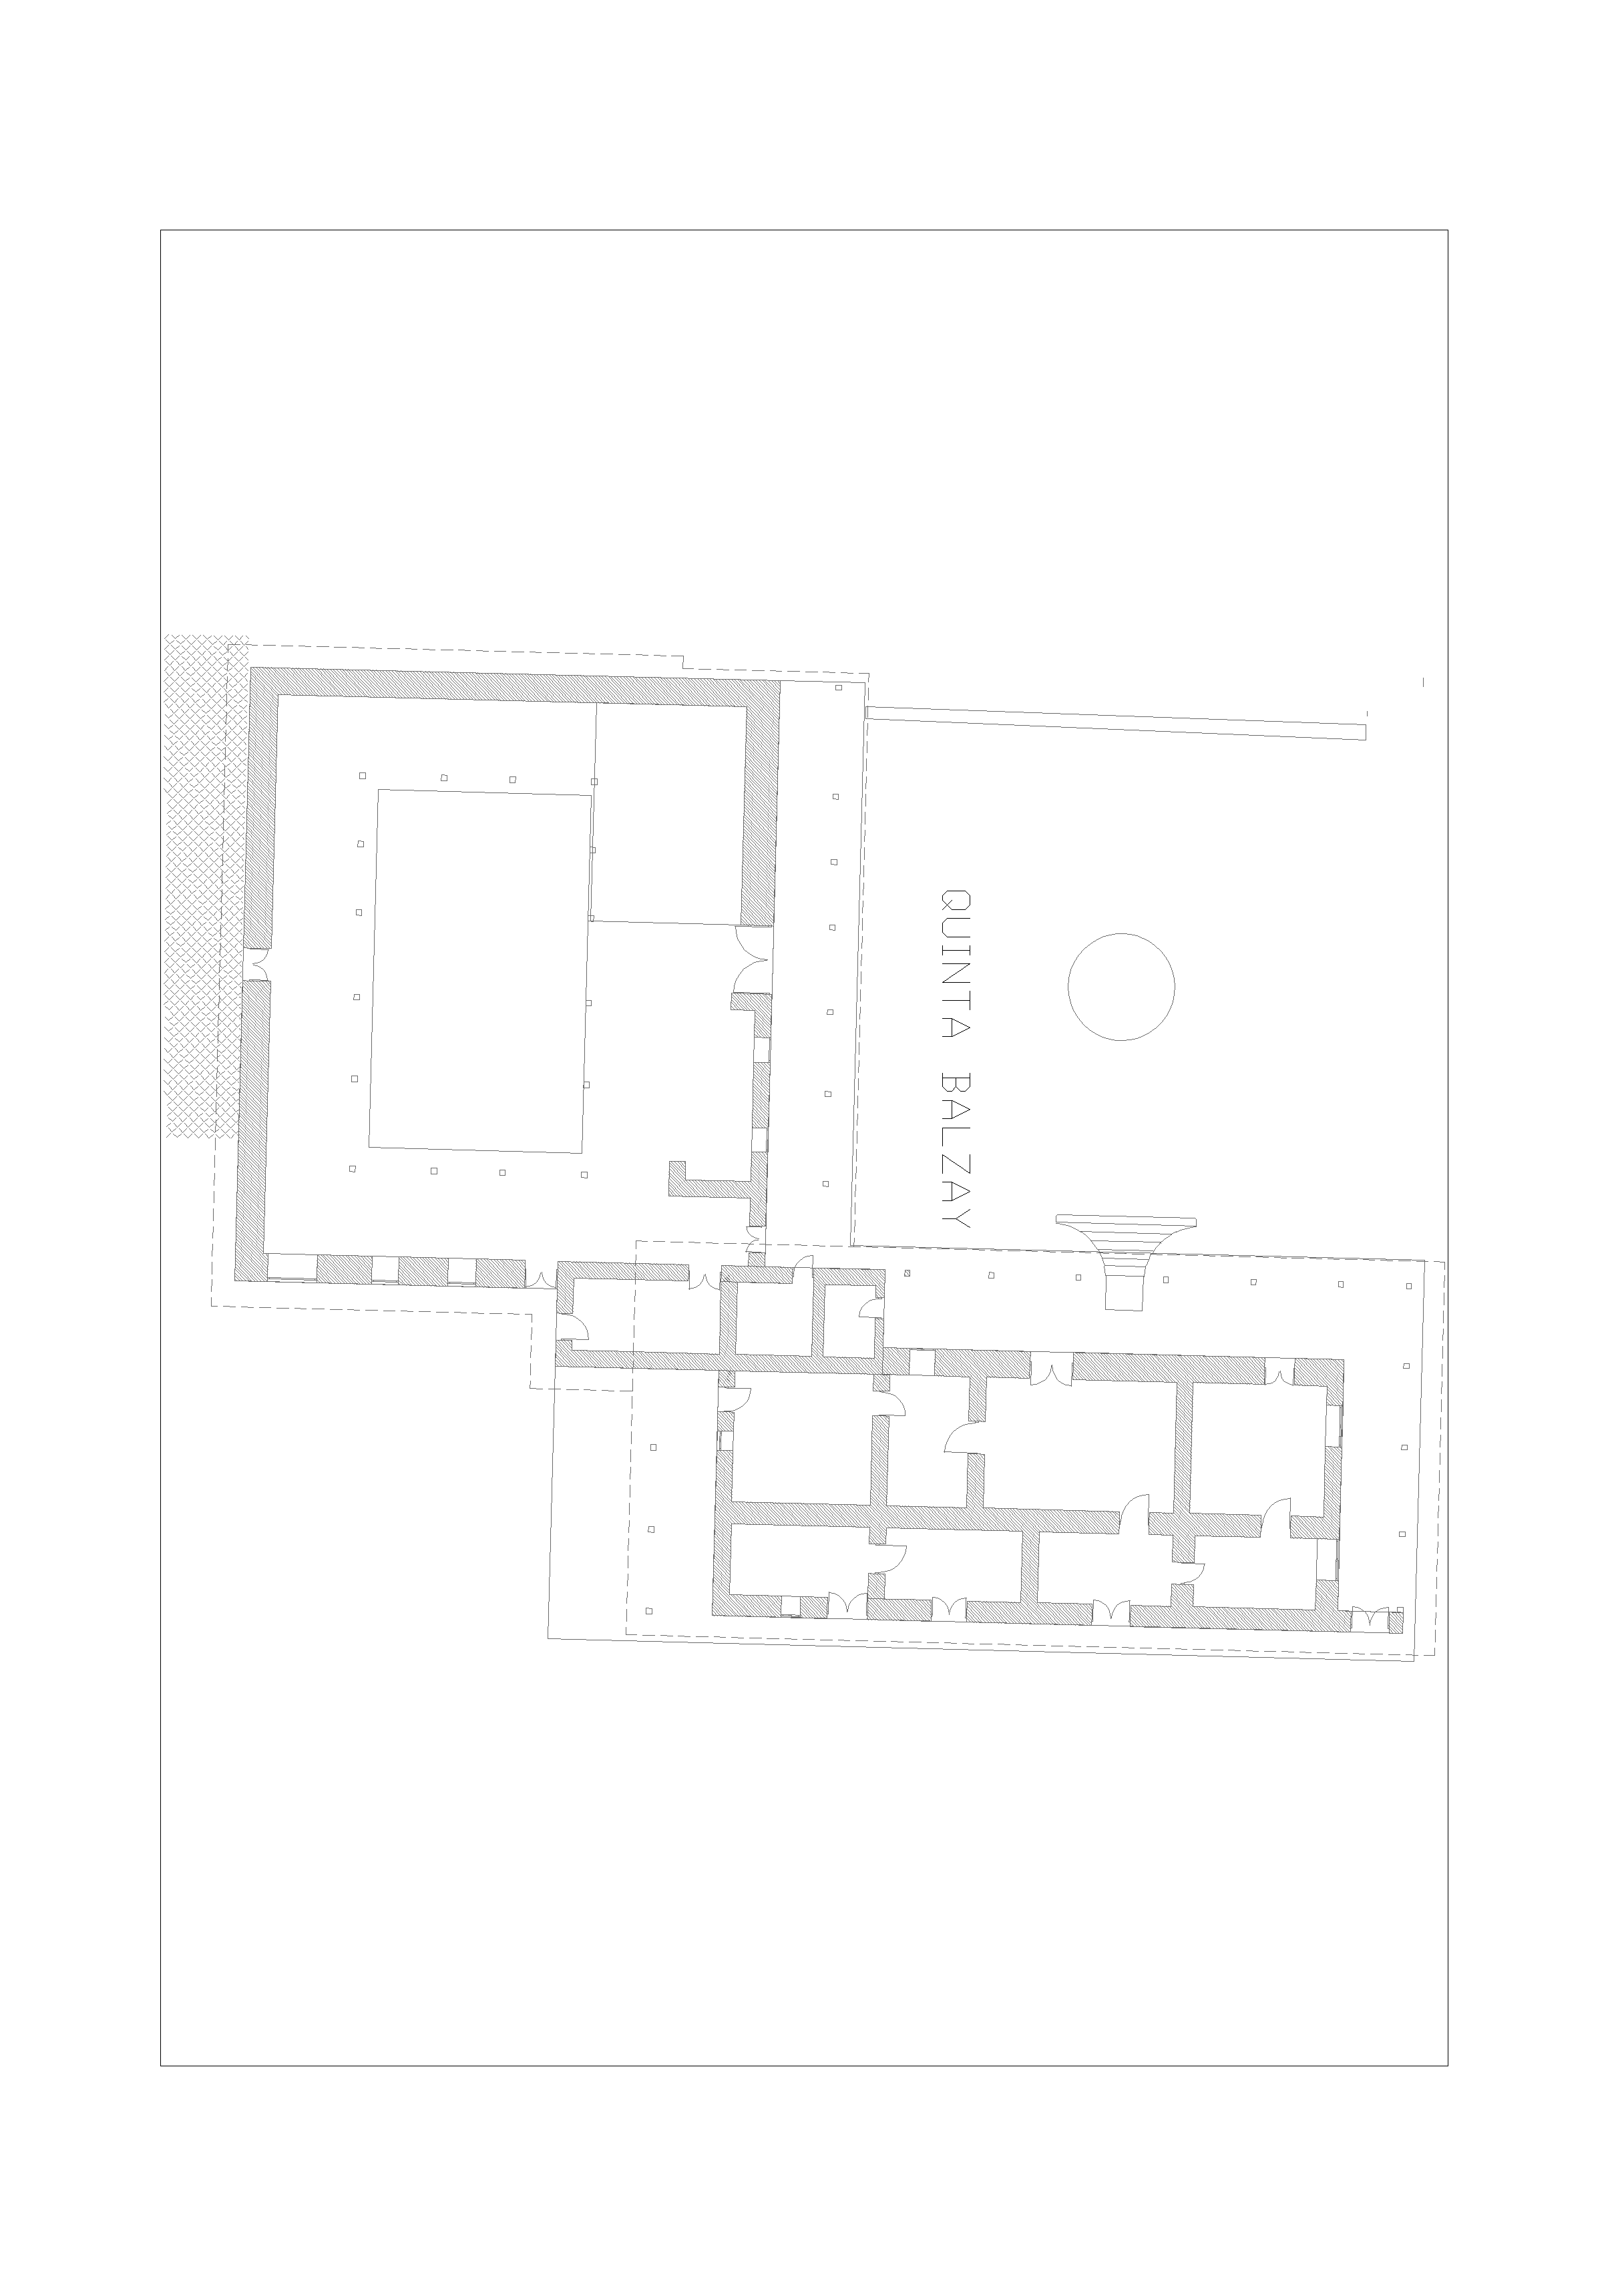
\includegraphics[width=0.92\linewidth,height=2.55cm,keepaspectratio]{../assets/plans/quintaBalzay.png}
        };
      \end{tikzpicture}
    \end{center}
    \vspace{0.15cm}
    {\footnotesize\color{MutedGray}\textbf{Escala 1:} comprender el campus como sistema de bloques y trayectos.}

    \column{0.49\textwidth}
    \begin{center}
      \begin{tikzpicture}
        \node[
          rounded corners=20pt,
          draw=LineGray,
          fill=white,
          inner sep=8pt
        ] {
          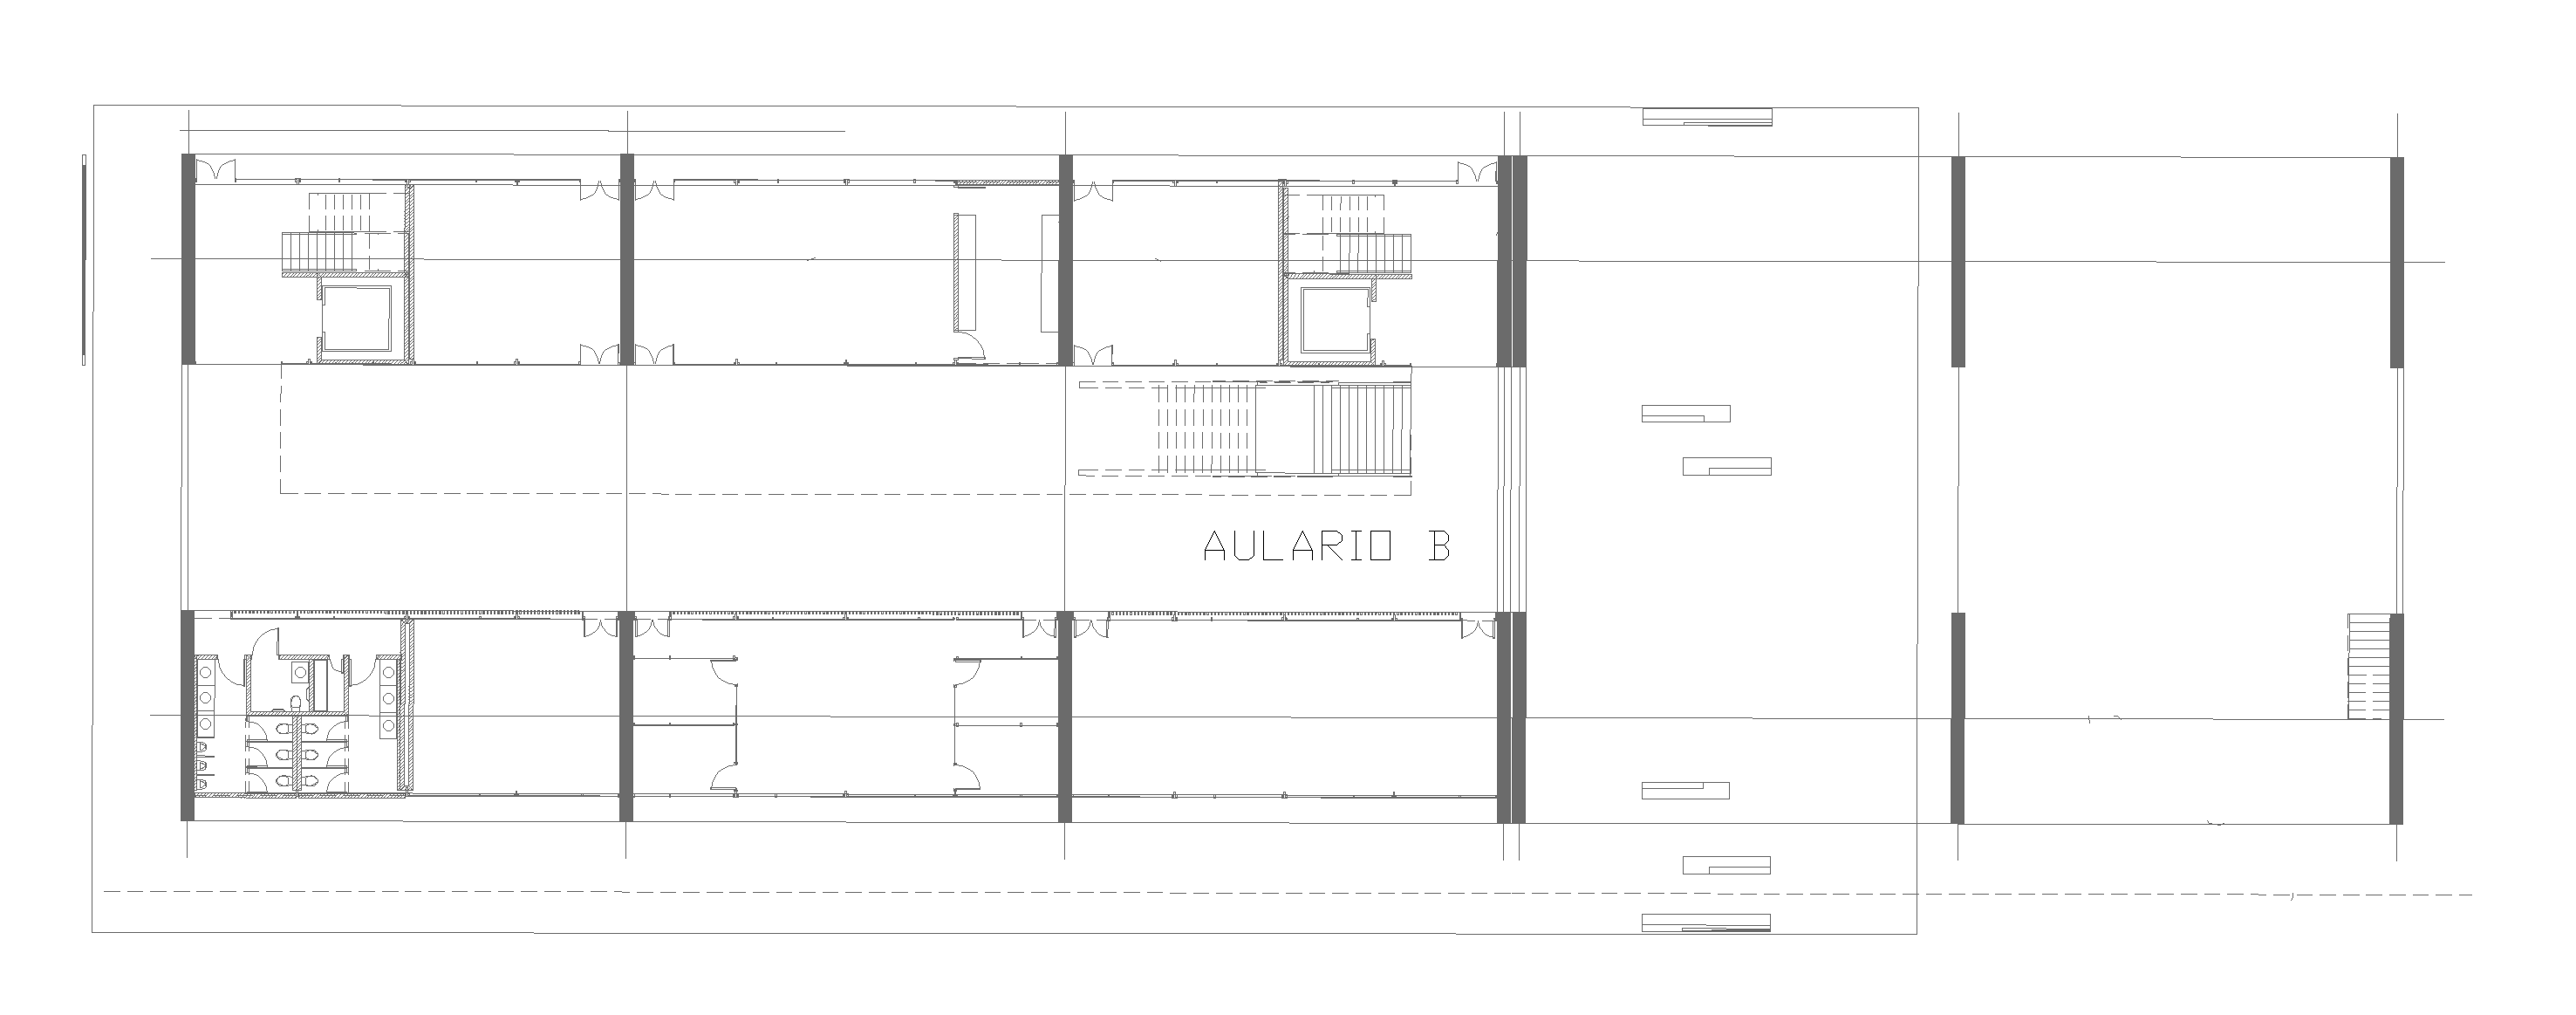
\includegraphics[width=0.92\linewidth,height=2.55cm,keepaspectratio]{../assets/plans/bloque_b_planta1.png}
        };
      \end{tikzpicture}
    \end{center}
    \vspace{0.15cm}
    {\footnotesize\color{MutedGray}\textbf{Escala 2:} abrir la planta correcta y resaltar el aula dentro del edificio.}
  \end{columns}

  \vspace{0.08cm}
  \begin{tikzpicture}
    \node[
      rounded corners=18pt,
      draw=FlutterLight,
      fill=FlutterLight!10,
      inner sep=11pt,
      text width=0.96\linewidth,
      align=left
    ] {
      {\footnotesize\textbf{Lo importante aqui no es la imagen, sino el modelo:} los espacios se alimentan desde datos editables, lo que permite ampliar edificios y aulas sin rehacer la interfaz.}
    };
  \end{tikzpicture}
\end{frame}

\begin{frame}{ }
  \frameheader{DEMO}{Navegando entre plantas de un edificio}
  \begin{center}
  \vspace{0.1cm}
  \movie[externalviewer]{
\includegraphics[width=9cm]{frames/navegacion_plantas/0.png}}{VIDEOS/Ejemplo_navegaciontentreplantas.mp4}
  \end{center}
\end{frame}

\begin{frame}[shrink=2]{ }
  \frameheader{DECISIONES}{Lo que de verdad cambio la experiencia}

  \begin{columns}[T,onlytextwidth]
    \column{0.48\textwidth}
    \simplecard{SoftGray}{0.88\linewidth}{{\small\textbf{1. Priorizar la busqueda}\\Si el usuario ya sabe el aula, no deberia explorar de mas.}}

    \vspace{0.08cm}
    \simplecard{white}{0.88\linewidth}{{\small\textbf{2. Separar perfiles}\\Un visitante necesita llegar; un estudiante necesita volver todos los dias.}}

    \vspace{0.08cm}
    \simplecard{SoftGray}{0.88\linewidth}{{\small\textbf{3. Mantener datos editables}\\JSON y planos permiten crecer sin bloquear el producto.}}

    \column{0.48\textwidth}
    \simplecard{white}{0.88\linewidth}{{\small\textbf{4. Publicar tambien en web}\\En eventos o campus nuevos, abrir un link rapido importa mas que instalar.}}

    \vspace{0.08cm}
    \simplecard{SoftGray}{0.88\linewidth}{{\small\textbf{5. No saturar la primera pantalla}\\Primero orientacion, luego capas de valor como horario, favoritos y tareas.}}

    \vspace{0.08cm}
    \begin{tikzpicture}
      \node[
        rounded corners=18pt,
        fill=FlutterDark,
        text=white,
        inner sep=10pt,
        text width=0.88\linewidth,
        align=left
      ] {
        {\scriptsize\textbf{Idea practica:} cuando el problema es espacial, la experiencia debe explicar el lugar antes de pedirle al usuario que entienda la app.}
      };
    \end{tikzpicture}
  \end{columns}
\end{frame}

\begin{frame}{ }
  \frameheader{DEMO}{Accesibilidad: modo oscuro y texto grande}
  \begin{center}
  \vspace{0.1cm}
  \movie[externalviewer]{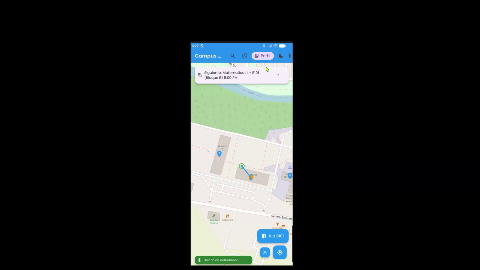
\includegraphics[width=9cm]{frames/accesibilidad/0.png}}{VIDEOS/Ejemplo_accesibilidad_modooscuro-texto.mp4}
  \end{center}
\end{frame}

\begin{frame}[shrink=5]{ }
  \frameheader{POR QUE FLUTTER}{Velocidad, alcance y buenas practicas}

  \begin{columns}[T,onlytextwidth]
    \column{0.48\textwidth}
    \simplecard{SoftGray}{0.88\linewidth}{{\small\textbf{Una sola base}\\El mismo producto funciona en varias plataformas.}}

    \vspace{0.08cm}
    \simplecard{white}{0.88\linewidth}{{\small\textbf{Iteracion visual}\\Ajustar pantallas y flujo fue rapido desde el inicio.}}

    \vspace{0.08cm}
    \simplecard{white}{0.88\linewidth}{{\small\textbf{Consistencia}\\La experiencia se siente igual en distintos dispositivos.}}

    \column{0.48\textwidth}
    \simplecard{FlutterLight!10}{0.88\linewidth}{{\small\textbf{Despliegue util}\\Web para acceso inmediato y apps para escenarios recurrentes.}}

    \vspace{0.08cm}
    \simplecard{FlutterBlue!10}{0.88\linewidth}{{\small\textbf{Ecosistema suficiente}\\Mapas, geolocalizacion, persistencia y UI estuvieron listos para integrarse.}}

    \vspace{0.12cm}
    \simplecard{SoftGray}{0.88\linewidth}{{\scriptsize\textbf{Paquetes y patrones aplicados}\\\textbf{Provider}, \textbf{Material~3}, \textbf{geolocator}, \textbf{flutter\_map}, \textbf{shared\_preferences}; datos en \textbf{JSON} y una sola base para web, movil y escritorio.}}
  \end{columns}
\end{frame}

\begin{frame}[shrink=12]{ }
  \frameheader{BUENAS PRACTICAS}{Reglas que seguimos para crecer sin romper}

  \begin{columns}[T,onlytextwidth]
    \column{0.49\textwidth}
    \simplecard{SoftGray}{0.9\linewidth}{{\scriptsize\textbf{Separar por responsabilidad}\\Cada parte quedo en su lugar: \textbf{screens} para flujo, \textbf{services} para datos y logica, y \textbf{widgets} para piezas reutilizables.}}

    \vspace{0.06cm}
    \simplecard{white}{0.9\linewidth}{{\scriptsize\textbf{Widgets pequenos y claros}\\Preferimos \textbf{StatelessWidget} cuando es posible, usamos \textbf{const} y evitamos meter logica de negocio dentro de \textbf{build()}.}}

    \vspace{0.06cm}
    \simplecard{FlutterLight!10}{0.9\linewidth}{{\scriptsize\textbf{Cierre con calidad}\\Estados y errores visibles, nombres consistentes y cierre siempre con \textbf{analyze}, \textbf{test} y \textbf{format}.}}

    \column{0.47\textwidth}
    \begin{tikzpicture}[
      node distance=0.14cm,
      root/.style={
        rounded corners=10pt, draw=FlutterBlue, fill=FlutterBlue!15,
        text width=3.4cm, align=center,
        font=\scriptsize\bfseries, text=FlutterDark, inner sep=5pt
      },
      folder/.style={
        rounded corners=6pt, draw=LineGray, fill=SoftGray,
        text width=3.4cm, align=left, font=\tiny, inner sep=3pt
      },
      link/.style={-{Latex[length=1.5mm]}, FlutterBlue, thick}
    ]
      \node[root] (lib) {lib/};
      \node[folder, below=of lib] (sc)
        {\textbf{screens/}\\{\color{MutedGray}vistas: mapa, bloque, planta, horario, tareas}};
      \node[folder, below=of sc]  (sv)
        {\textbf{services/}\\{\color{MutedGray}logica: rutas, favoritos, horario, aulas, tema}};
      \node[folder, below=of sv]  (mo)
        {\textbf{models/}\\{\color{MutedGray}estructuras: roles, bloques y aulas}};
      \node[folder, below=of mo]  (wi)
        {\textbf{widgets/}\\{\color{MutedGray}UI: rutas animadas, distancia, trayecto}};
      \node[folder, below=of wi]  (se)
        {\textbf{search/}\\{\color{MutedGray}busqueda de aulas por nombre}};
      \node[folder, below=of se]  (da)
        {\textbf{data/}\\{\color{MutedGray}campus\_data: ubicacion de aulas}};
      \draw[link] (lib)--(sc); \draw[link] (sc)--(sv); \draw[link] (sv)--(mo);
      \draw[link] (mo)--(wi); \draw[link] (wi)--(se); \draw[link] (se)--(da);
    \end{tikzpicture}
  \end{columns}
\end{frame}

\begin{frame}[shrink=3]{ }
  \frameheader{APRENDIZAJES}{Lo que me dejo construir esta app}

  \begin{columns}[T,onlytextwidth]
    \column{0.5\textwidth}
    {\scriptsize
    \begin{itemize}
      \item Un problema pequeno y concreto suele producir un mejor producto inicial.
      \item La capa de datos importa tanto como la interfaz.
      \item En navegacion, \textbf{claridad} vale mas que sofisticacion.
      \item Pensar en perfiles cambia la experiencia final.
    \end{itemize}
    }

    \column{0.46\textwidth}
    \begin{tikzpicture}
      \node[
        rounded corners=22pt,
        draw=FlutterDark,
        fill=FlutterDark,
        text=white,
        inner sep=11pt,
        text width=0.92\linewidth,
        align=left
      ] {
        {\scriptsize\textbf{Aprendizaje central}\\Flutter fue importante, pero el verdadero salto fue pensar la app como una experiencia de llegada, no solo como un visor de mapas.}
      };
    \end{tikzpicture}

    \vspace{0.16cm}
    \begin{tikzpicture}
      \node[
        rounded corners=18pt,
        draw=LineGray,
        fill=SoftGray,
        inner sep=8pt,
        text width=0.92\linewidth,
        align=left
      ] {
        {\scriptsize\textbf{Valor para la charla}\\Este proyecto muestra que Flutter tambien es una herramienta potente para resolver necesidades locales, universitarias y muy concretas.}
      };
    \end{tikzpicture}
  \end{columns}
\end{frame}

\begin{frame}{ }
  \frameheader{DEMO}{Estudiante gestionando sus tareas}
  \begin{center}
  \vspace{0.1cm}
  \movie[externalviewer]{
\includegraphics[width=9cm]{frames/estudiante_tasks/0.png}}{VIDEOS/Ejemplo_Estudiante_tasks.mp4}
  \end{center}
\end{frame}

\begin{frame}{ }
  \frameheader{SIGUIENTE PASO}{Hacia donde puede crecer UNIMAP}

  \begin{center}
  \begin{tikzpicture}[node distance=0.35cm]
    \node[
      rounded corners=18pt,
      draw=LineGray,
      fill=white,
      minimum width=2.95cm,
      minimum height=1.75cm,
      align=center,
      inner sep=8pt
    ] (r1) {Mas edificios\\y mas plantas};

    \node[right=of r1,
      rounded corners=18pt,
      draw=LineGray,
      fill=SoftGray,
      minimum width=2.95cm,
      minimum height=1.75cm,
      align=center,
      inner sep=8pt
    ] (r2) {Onboarding\\para primer ingreso};

    \node[right=of r2,
      rounded corners=18pt,
      draw=LineGray,
      fill=white,
      minimum width=2.95cm,
      minimum height=1.75cm,
      align=center,
      inner sep=8pt
    ] (r3) {Indicaciones\\mas precisas};

    \node[right=of r3,
      rounded corners=18pt,
      draw=LineGray,
      fill=SoftGray,
      minimum width=2.95cm,
      minimum height=1.75cm,
      align=center,
      inner sep=8pt
    ] (r4) {Feedback y\\analitica de uso};

    \draw[-{Latex[length=3mm]},very thick,FlutterBlue] (r1.east) -- (r2.west);
    \draw[-{Latex[length=3mm]},very thick,FlutterBlue] (r2.east) -- (r3.west);
    \draw[-{Latex[length=3mm]},very thick,FlutterBlue] (r3.east) -- (r4.west);
  \end{tikzpicture}
  \end{center}

  \vspace{0.45cm}
  \begin{tikzpicture}
    \node[
      rounded corners=18pt,
      draw=FlutterLight,
      fill=FlutterLight!10,
      inner sep=12pt,
      text width=0.96\linewidth,
      align=left
    ] {
      \textbf{Vision:} que orientarse dentro de la universidad deje de ser una barrera invisible, especialmente para quienes recien llegan o visitan un campus por primera vez.
    };
  \end{tikzpicture}
\end{frame}

{
\setbeamertemplate{footline}{}
\begin{frame}[plain]
  \begin{tikzpicture}[remember picture,overlay]
    \fill[FlutterNavy] (current page.south west) rectangle (current page.north east);
    \fill[FlutterBlue] (current page.south west) rectangle ([xshift=3.9cm]current page.north west);
    \fill[FlutterLight,opacity=.18] ([xshift=.82\paperwidth,yshift=.18\paperheight]current page.south west) circle (1.65cm);
    \fill[FlutterLight,opacity=.10] ([xshift=.74\paperwidth,yshift=.77\paperheight]current page.south west) circle (2.15cm);
  \end{tikzpicture}

  \begin{minipage}[t][0.95\textheight][c]{0.63\linewidth}
    {\fontsize{30}{34}\selectfont\bfseries\color{white}Gracias\par}
    \vspace{0.24cm}
    {\large\color{white!90}Flutter tambien puede resolver problemas muy cercanos, muy cotidianos y muy locales.\par}

    \vspace{0.56cm}
    {\large\color{FlutterLight}\textbf{UNIMAP}}\par
    {\normalsize\color{white!90}Navegacion universitaria multiplataforma para el campus\par}

    \vspace{0.32cm}
    {\small\color{white!80}\textbf{Jean Aucapina}\par}
    {\scriptsize\color{FlutterLight!80}Preguntas, codigo y demo: despues de la charla\par}

    \vfill
    
\includegraphics[height=0.56cm]{imagenes/flutterlogo.png}\hspace{0.20cm}
    
\includegraphics[height=0.56cm]{imagenes/ucuencalogo.png}
  \end{minipage}\hfill
  \begin{minipage}[t][0.95\textheight][c]{0.31\linewidth}
    \begin{center}
      \begin{tikzpicture}
        \node[
          rounded corners=24pt,
          fill=white,
          inner sep=10pt
        ] {
\includegraphics[width=0.74\linewidth]{../assets/plans/ico.png}};
      \end{tikzpicture}
    \end{center}
  \end{minipage}
\end{frame}
}

\end{document}
